%========================================================================================
% TU Dortmund, Informatik Lehrstuhl VII
%========================================================================================

\chapter{Vom Höchstspannungsnetz zum Graphen}
\label{Kapitel 2}
%

\section{Höchstspannungsnetz}
\label{Höchstspannungsnetz}
%
\begin{figure}[t]
	\centering
	{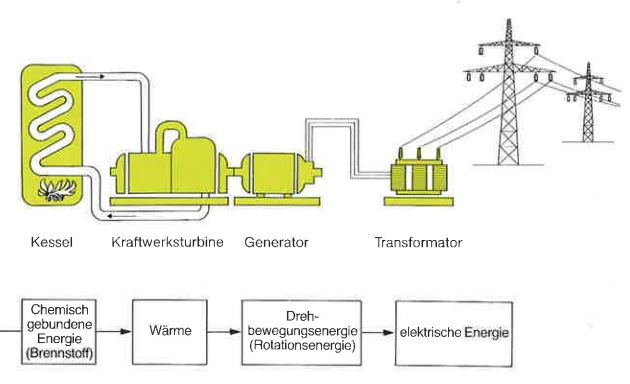
\includegraphics[scale=0.9]{bilder/pds}\label{fig_pds}
	}\\
	\caption[Prinzip der Stromerzeugung]{Prinzip der Stromerzeugung[1]}
	\label{fig_pds}
\end{figure}
\begin{figure}[t]
	\centering
	{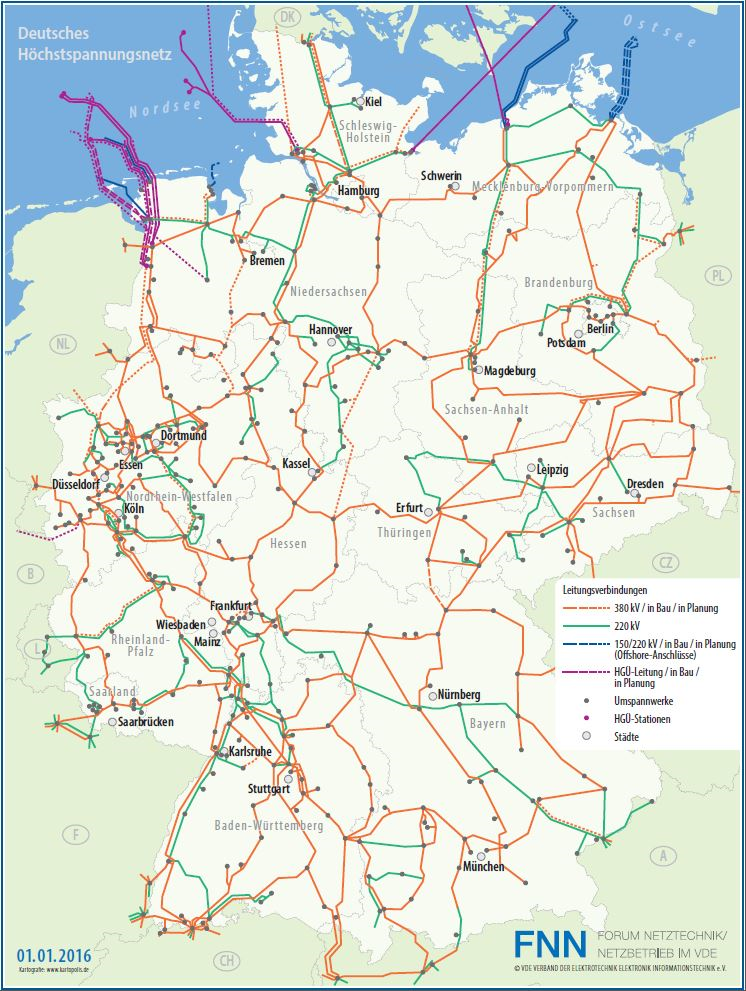
\includegraphics[scale=0.5]{bilder/hochstspannungsnetz}\label{fig_hochstspannungsnetz}
	}\\
	\caption[Karte des deutschen Höchstspannungsnetzes]{Karte des deutschen Höchstspannungsnetzes}
	\label{fig_hochstspannungsnetz2}
\end{figure}
\begin{figure}[t]
	\centering
	{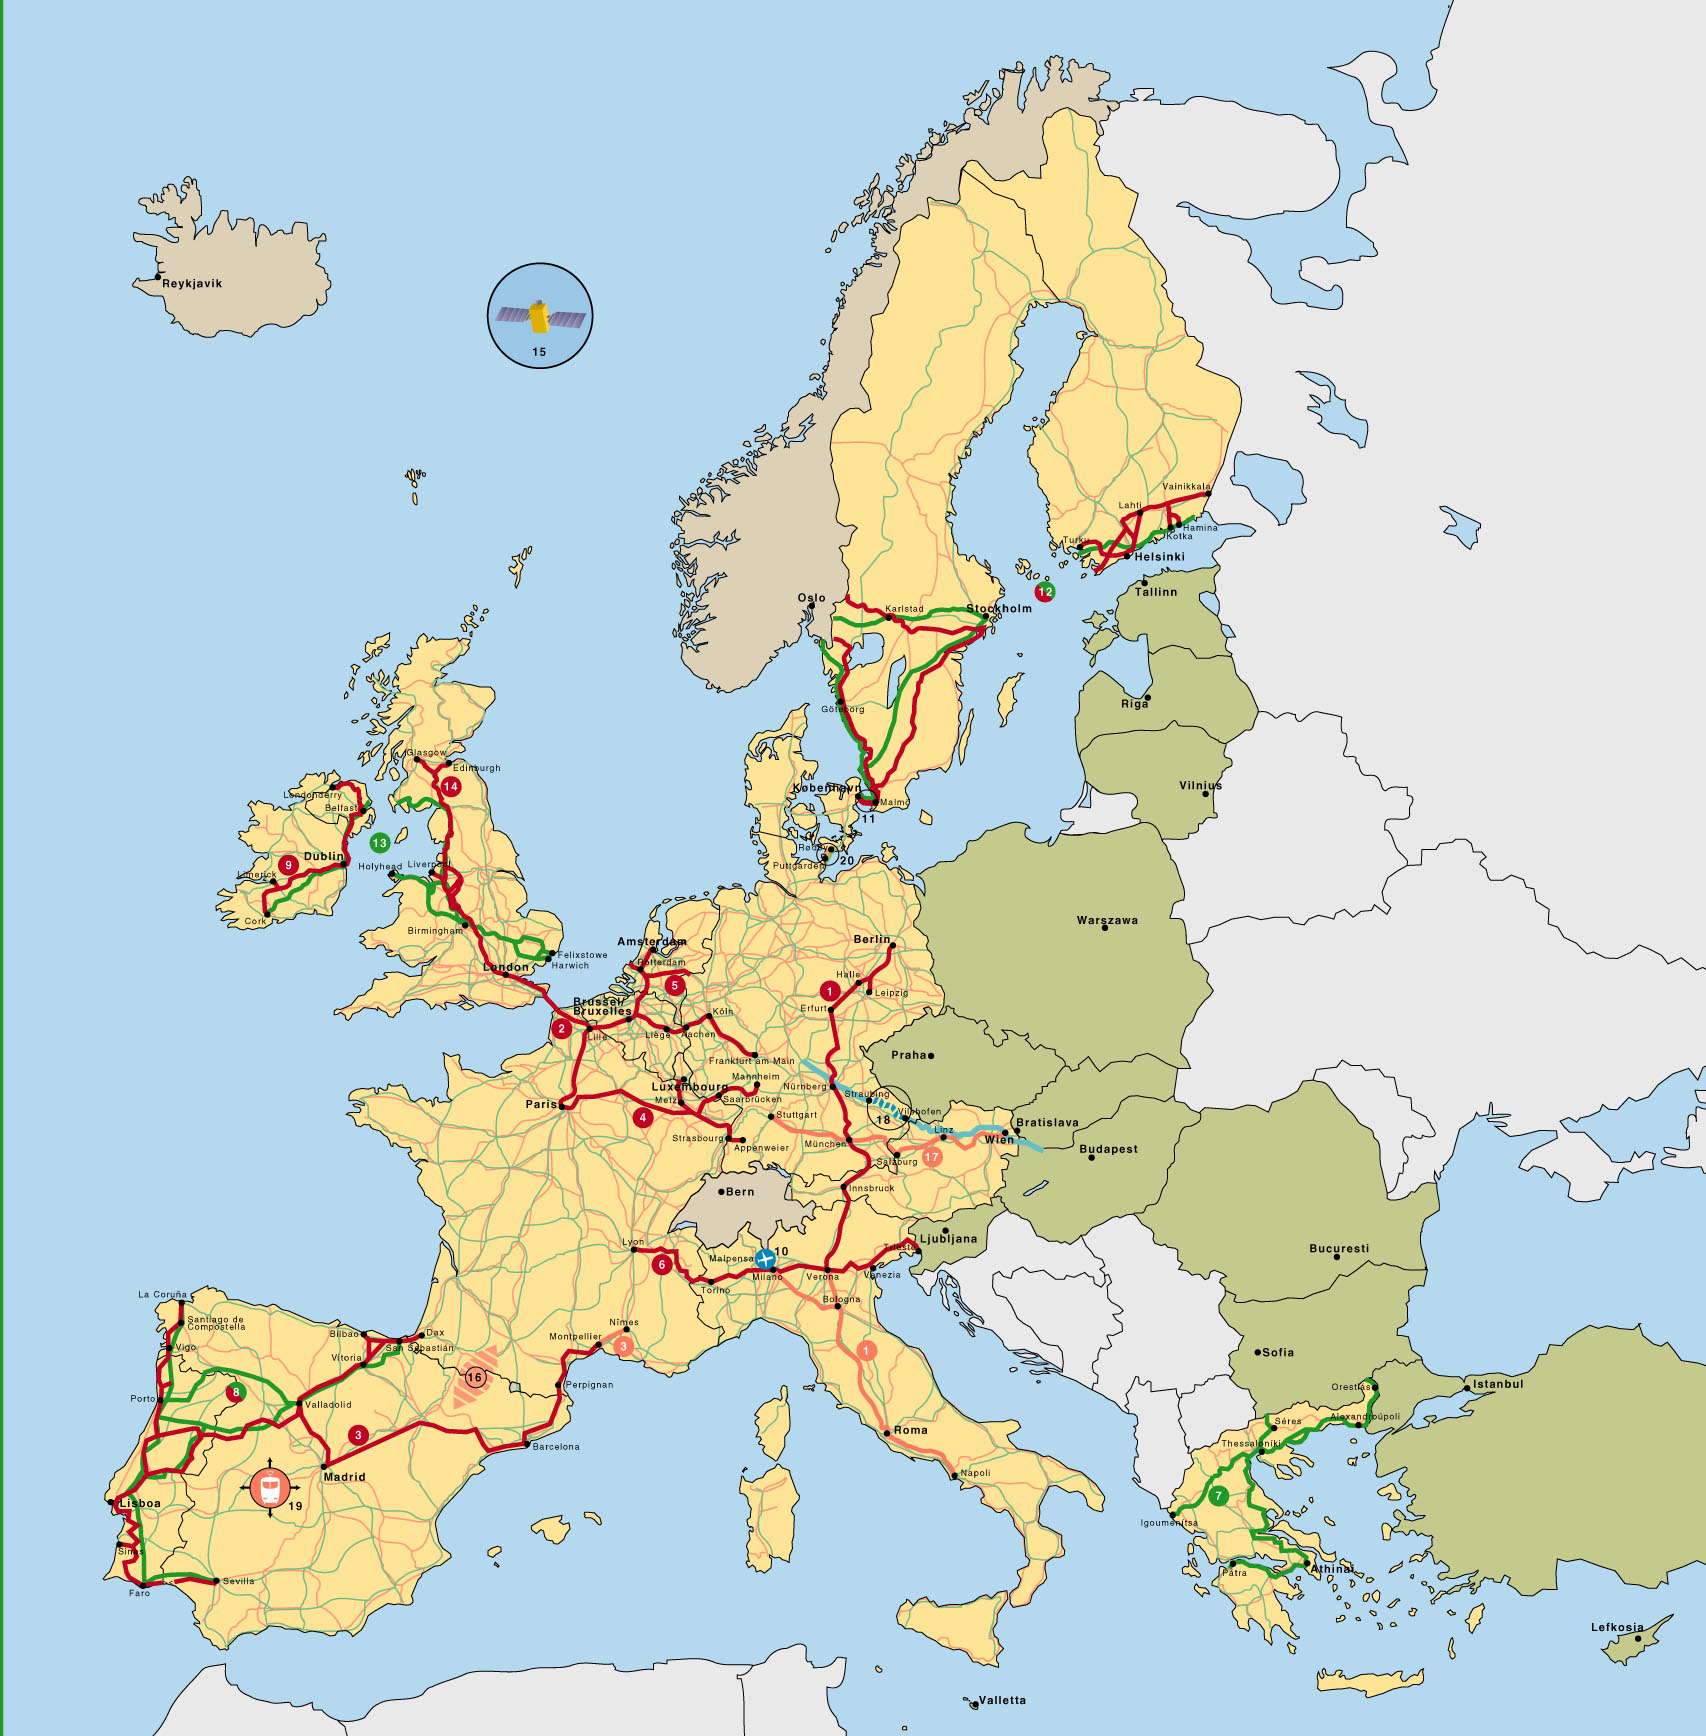
\includegraphics[scale=0.9]{bilder/europastromnetz}\label{fig_europastromnetz}
	}\\
	\caption[Karte des europäischen Verbundnetzes]{Karte des europäischen Verbundnetzes}
	\label{fig_europastromnetz}
\end{figure}
Um elektrische Energie über große Distanzen zu transportieren werden Höchstspannungsnetze benutzt. Von einem Kraftwerk ausgehend wird versucht möglichst viele Haushalte, Industrie- und Gewerbebetriebe zu erreichen. Davon ausgehend wird auch der Standort der meisten Kraftwerke bestimmt. Einige Kraftwerke lassen sich nur an bestimmten Standorten errichten, zum Beispiel ein Wasserkraftwerk muss an einem Fluss oder Staudamm errichtet werden. So ist es oft nicht möglich genug Verbraucher zu erreichen, sodass es Mittel bedarf den elektrischen Strom auch über weite Strecken hinweg zu transportieren.

Die Generatoren der modernen Kraftwerke erzeugen eine Spannung von $10500 V$, $21000V$ oder $27000V$[1]. Die Höhe dieser Spannung ist bestimmt durch die Größe bzw. die Leistungsfähigkeit des Kraftwerks und somit von der Nennleistung des Generators.

Da der überwiegende Teil der elektrischen Energie in Wärmekraftwerken erzeugt wird und diese mit einer Generatorleistung von $600$ bis $1300MW$, bedeutet dies, dass Ströme zwischen $15000A$ und $30000A$ abgegeben werden müssen. Das ist jedoch weder aus technischen noch wirtschaftlichen Gründen für einen Transport über lange Distanzen lohnenswert, da es entweder sehr großen Leiterquerschnitte oder sehr große Stromverluste zur Folge hätte.

Es kann die gleiche Leistung $P$ auch mit weniger Strom $I$ und einer erhöhten Spannung $U$ erreicht werden, denn die Beziehung lautet:

\begin{align}
	P = U \cdot I
\end{align}  

Diese Eigenschaft wird ausgenutzt und das führt dazu, dass die Generatorspannung bereits direkt am Kraftwerk durch einen Transformator in eine höhere Spannung umgeformt wird. Dadurch wird die elektrische Leistung mit kleineren Stromstärken über die Netze geleitet. Nur die Übertragung in höheren Spannungen ermöglicht es die elektrische Energie effizient zu übertragen. Die Anpassungen führen zu einem sehr geringen Gesamtverlust von etwa $5\%$ der erzeugten Energie. 

Die erforderlichen Leitungen um ein effizientes Netz sicherzustellen werden in verschiedenen Ebenen anhand ihrer Betriebsspannung eingeteilt:
\begin{itemize}
	\item Höchstspannungsleitungen mit Betriebsspannungen über $150000V$
	\item Hochspannungsleitungen mit Betriebsspannungen über $60000V$
	\item Mittelspannungsleitungen mit Betriebsspannungen über $1000V$
	\item Niederspannungsleitungen mit Betriebsspannungen bis $1000V$.
\end{itemize} 

In Deutschland werden die Höchstspannungsleitungen mit $380 000V$ oder mit $220 000V$ betrieben. Sie sind zuständig für die überregionale Übertragung. Von den Kraftwerken werden mittels Höchstspannungsleitungen Umspannanlagen, die in der Nähe der Verbraucherschwerpunkte liegen verbunden. In den Umspannanlagen findet eine Herabtransformation auf $110 000V$ statt. Dann sind Hochspannungsleitungen für die weitere regionale Übertragung zuständig. Nach einer weiteren Herabtransformation in einer Umspannanlage beträgt die Spannung noch $10 000V$ oder $20 000V$ und ist jetzt bereit für die Übertragung in der Stadt mittels Mittelspannungsleitungen.

Um die Transportaufgaben zu bewältigen müssen die Höchstspannungsleitungen oft über 100 km lang sein. Das komplette Netz, welches sich über Deutschland erstreckt wird auch das Verbundnetz genannt. Die Einzelnetze werden dabei über Kuppelstellen miteinander verbunden. Das Netz erstreckt sich nicht nur über Deutschland sondern über ganz Europa. Der Vorteil bei einem großen verbundenen Netz sind der Nutz- und Erzeugungsausgleich sowie der kostengünstigen Reservestellung für nicht verbundene Kraftwerke[1].

Da der Stromverbrauch stets variabel ist und sehr örtlich sowie zeitlich unterschiedlich, macht ein großes Verbundnetz viel Sinn. Ebenso aus Sicht der Kraftwerke, zum Beispiel wenn der Schneefall oder Regen ausbleibt, so gibt es an einem Kraftwerk welches an einem Staudamm oder Fluss errichtet worden ist weniger Energie und der Bedarf kann leicht durch andere Quellen über das Netz gedeckt werden.\newline

Es gibt zwei verschiedene Arten für den Transport der elektrischen Energie:
\begin{itemize}
	\item Freileitung
	\item Kabel.
\end{itemize} 
Entschieden wird anhand der technischen Möglichkeiten, die unterschiedlichen physikalischen Eigenschaften der Freileitungen und Kabel, die Kosten sowie Vorstellungen hinsichtlich des Landschaftsschutzes und der Gestaltung des Stadtbildes[1].

Die meisten Leiter bestehen aus Kupfer und Aluminium, dank der hohen Elastizität und elektrischen Leitfähigkeit. Aluminium hat gerade für den Freileitungsbau eine besondere Eigenschaft des sehr geringen Eigengewichtes, was einen größeren Abstand der Masten ermöglicht.

Die Kabel bestehen aus einem Kern der Leiter, welche voneinander durch Isolierungen geschützt werden. Diese nennt man Adern. Mehrere Adern gebunden durch einen Mantel ergeben das letztendliche Kabel, diese können durch ein- oder mehradrig unterschieden werden. Die einzelnen Isolierungen der Adern bestehen aus ölgetränkten Papier, bei niedrigen Spannungen auch Kunststoff(PVC). Die dicke der Isolierung wird durch die jeweilige Nennspannung der Adern bestimmt.

Der Mantel soll die Kabel eng zusammenhalten und gegen äußere mechanische Beschädigungen schützen, ebenso muss er gegen eindringende Feuchtigkeit isolieren. Da Hochspannungsleitungen eine besonders große Isolierung benötigen, werden die Leiter in einem Stahlrohr mit Stickstoffgas unter sehr großen Druck verlegt.


\section{Graph}
\label{Graph}
%
Ein Graph ist eine Struktur, die Informationen über zusammenhängende Objekte repräsentiert. Die jeweiligen Objekte werden Knoten und deren Verbindungen Kanten genannt.
Somit hat ein Graph eine Menge von Knoten und Kanten.
\begin{lstlisting}[style=C++, caption=Struktur des Graphen]{Name}
class Graph {
List<Knoten> knoten;
List<Kante> kanten;
}
\end{lstlisting}
Ein Knoten besteht aus einem Koordinatenpaar $(x,y)$, welches definiert wo der Knoten liegt.
\begin{lstlisting}[style=C++, caption=Struktur eines Knotens]{Name}
class Knoten {
int x,y;
public Knoten(int x, int y)
{	
this.x = x;
this.y = y;
}	
}
\end{lstlisting}
Die einzelnen Knoten werden über Kanten miteinander verbunden. Eine Kante speichert den Start- sowie Endknoten der Verbindung.
\begin{lstlisting}[style=C++, caption=Struktur eines Knotens]{Name}
class Knoten {
int x,y;
public Knoten(int x, int y)
{	
this.x = x;
this.y = y;
}	
}
\end{lstlisting}
Neue Knoten und Kanten können in der Graph-Klasse mit der Funktion $createKnoten()$ und $createKante()$ hinzugefügt werden. Diese Funktionen erstellen einen neuen Knoten beziehungsweise Kante und fügen sie der jeweiligen Liste hinzu.

Nun kann der Graph auf einer Oberfläche gezeichnet, indem erst die Knoten platziert werden anhand ihrer $x$ und $y$ Koordinate und anschließend die Kanten zwischen den jeweiligen Knoten. 


\section{Vom Höchstspannungsnetz zum Graphen}
\label{Vom Höchstspannungsnetz zum Graphen}
%

Es wurden zwei Schritte unternommen um aus dem Höchstspannungsnetz einen repräsentierenden Graphen zu bekommen. Zum einen wurden die jeweiligen Masten zu Knoten und jeweils eins ihrer Leiterseile zu einer verbindenden Kante. Die Position der Masten war aus einer Karte des Höchstspannungsnetz zu bekommen, ebenso deren Verbindungen. 

Da es besonders wichtig ist darzustellen wie viele einzelne Leiterseile über die jeweiligen Verbindungen laufen, musste dieses noch hinzugefügt werden. Es wurde für jedes Leiterseil welches über einen der Masten lief ein jeweiliger Knoten erstellt, und jeweils mit einer Kante verbunden. Diese zusätzlichen Knoten wurden direkt neben dem ursprünglichen Knoten verteilt. Nun hat man die wichtigsten Informationen des Netzes in einen Graphen übertragen.

Die Städte und Orte werden dabei als unbewegliche Knoten angelegt damit der resultierende Graph nicht zu sehr vom ursprünglichen abweicht. Jegliche Eckpunkte zwischen den Orten wurde mithilfe eines weiteren beweglichen Knotens modelliert.

\begin{figure}[t]
	\centering
	\subfigure[Ausschnit des deutschen Höchstspannungsnetzes. Die markierten Orte werden zu den Knoten und die Verbindungen werden zu den Kanten des Graphen.]
	{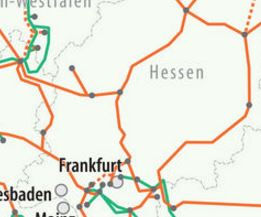
\includegraphics[scale=0.8]{bilder/kartenausschnitt}\label{fig_kartenausschnitt}
	}
	\hspace{1.0cm}%
	\subfigure[Den Ausschnitt der Karte als Graphen mit jeweils nur einer Leitung.]
	{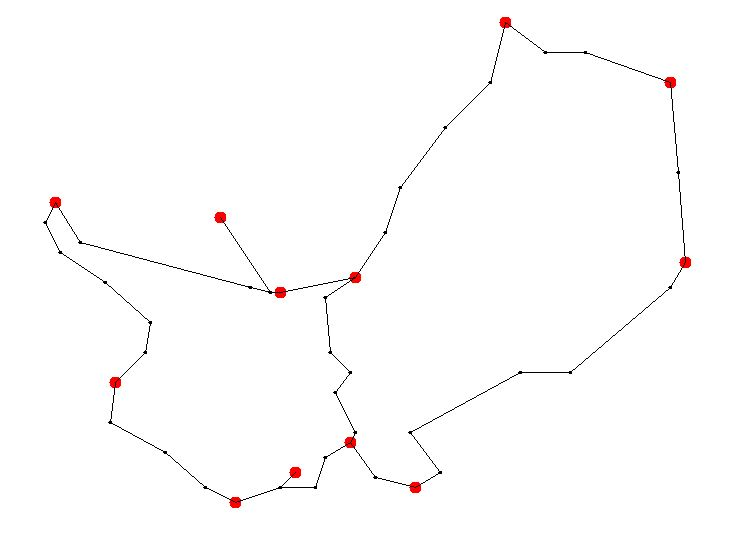
\includegraphics[scale=0.4]{bilder/ausschnittgraph}\label{fig_ausschnittgraph}
	}
	\hspace{1.0cm}%
	\subfigure[Die zusätzlichen Leitungen wurden neben dem eigentlichen Knoten hinzugefügt. Hier jeweils immer genau drei.]
	{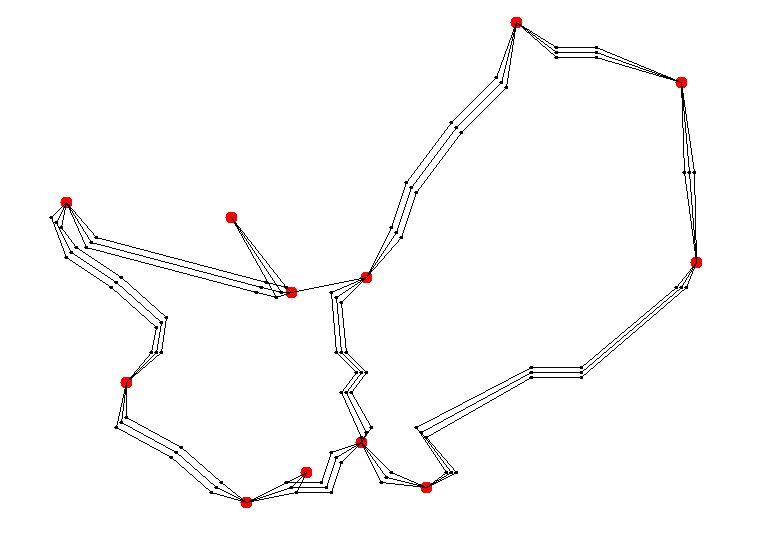
\includegraphics[scale=0.4]{bilder/ausschnittfertigergraph}\label{fig_ausschnittfertigergraph}
	}
	\\
	\caption[Das schrittweise Vorgehen um einen repräsentierenden Graphen zu erhalten]{Das schrittweise Vorgehen um einen repräsentierenden Graphen zu erhalten}
	\label{fig_testbild2}
\end{figure}